\documentclass[12pt,reqno,oneside]{amsart}
\usepackage{import}
%===============================%
%  Packages and basic settings  %
%===============================%
\usepackage[headheight=15pt,rmargin=0.5in,lmargin=0.5in,tmargin=0.75in,bmargin=0.75in]{geometry}
\usepackage{imakeidx}
\usepackage{framed}
\usepackage{amssymb}
\usepackage{amsmath}
\usepackage{mathrsfs}
\usepackage{enumitem}
\usepackage{hyperref}
\usepackage{appendix}
\usepackage[capitalise,noabbrev]{cleveref}
\usepackage{tikz}
\usepackage{tikz-cd}
\usepackage{nomencl}\makenomenclature
\usetikzlibrary{braids,arrows,decorations.markings,calc}

%====================================%
%  Theorems, environments & cleveref  %
%====================================%
\newtheorem{theorem}{Theorem}[section]
\newtheorem{proposition}{Proposition}[section]
\newtheorem{corollary}{Corollary}[section]
\newtheorem{lemma}{Lemma}[section]
\newtheorem{conjecture}{Conjecture}[section]
\newtheorem{remark}{Remark}[section]

\newenvironment{stabular}[2][1]
  {\def\arraystretch{#1}\tabular{#2}}
  {\endtabular}

%==================================%
%  Custom commands & environments  %
%==================================%
\newcommand{\legendre}[2]{\left(\frac{#1}{#2}\right)}
\newcommand{\dlegendre}[2]{\displaystyle{\left(\frac{#1}{#2}\right)}}
\newcommand{\tlegendre}[2]{\textstyle{\left(\frac{#1}{#2}\right)}}
\newcommand{\psum}{\sideset{}{'}\sum}
\newcommand{\asum}{\sideset{}{^{\ast}}\sum}
\newcommand{\tmod}[1]{\ \left(\text{mod }#1\right)}
\newcommand{\xto}[1]{\xrightarrow{#1}}
\newcommand{\xfrom}[1]{\xleftarrow{#1}}
\newcommand{\normal}{\mathrel{\unlhd}}
\newcommand{\mf}{\mathfrak}
\newcommand{\mc}{\mathcal}
\newcommand{\ms}{\mathscr}

\newcommand{\Mat}{\mathrm{Mat}}
\newcommand{\GL}{\mathrm{GL}}
\newcommand{\SL}{\mathrm{SL}}
\newcommand{\PSL}{\mathrm{PSL}}
\renewcommand{\O}{\mathrm{O}}
\newcommand{\SO}{\mathrm{SO}}
\newcommand{\U}{\mathrm{U}}
\newcommand{\Sp}{\mathrm{Sp}}

\newcommand{\N}{\mathbb{N}}
\newcommand{\Z}{\mathbb{Z}}
\newcommand{\Q}{\mathbb{Q}}
\newcommand{\R}{\mathbb{R}}
\newcommand{\C}{\mathbb{C}}
\newcommand{\F}{\mathbb{F}}
\renewcommand{\H}{\mathbb{H}}
\renewcommand{\P}{\mathbb{P}}

\renewcommand{\a}{\alpha}
\renewcommand{\b}{\beta}
\newcommand{\g}{\gamma}
\renewcommand{\d}{\delta}
\newcommand{\z}{\zeta}
\renewcommand{\t}{\theta}
\renewcommand{\i}{\iota}
\renewcommand{\k}{\kappa}
\renewcommand{\l}{\lambda}
\newcommand{\s}{\sigma}
\newcommand{\w}{\omega}

\newcommand{\G}{\Gamma}
\newcommand{\D}{\Delta}
\renewcommand{\L}{\Lambda}
\newcommand{\W}{\Omega}

\newcommand{\e}{\varepsilon}
\newcommand{\vt}{\vartheta}
\newcommand{\vphi}{\varphi}
\newcommand{\emt}{\varnothing}

\newcommand{\x}{\times}
\newcommand{\ox}{\otimes}
\newcommand{\op}{\oplus}
\newcommand{\bigox}{\bigotimes}
\newcommand{\bigop}{\bigoplus}
\newcommand{\del}{\partial}
\newcommand{\<}{\langle}
\renewcommand{\>}{\rangle}
\newcommand{\lf}{\lfloor}
\newcommand{\rf}{\rfloor}
\newcommand{\wtilde}{\widetilde}
\newcommand{\what}{\widehat}
\newcommand{\conj}{\overline}
\newcommand{\cchi}{\conj{\chi}}

\DeclareMathOperator{\id}{\textrm{id}}
\DeclareMathOperator{\sgn}{\mathrm{sgn}}
\DeclareMathOperator{\im}{\mathrm{im}}
\DeclareMathOperator{\rk}{\mathrm{rk}}
\DeclareMathOperator{\tr}{\mathrm{trace}}
\DeclareMathOperator{\nm}{\mathrm{norm}}
\DeclareMathOperator{\ord}{\mathrm{ord}}
\DeclareMathOperator{\Hom}{\mathrm{Hom}}
\DeclareMathOperator{\End}{\mathrm{End}}
\DeclareMathOperator{\Aut}{\mathrm{Aut}}
\DeclareMathOperator{\Tor}{\mathrm{Tor}}
\DeclareMathOperator{\Ann}{\mathrm{Ann}}
\DeclareMathOperator{\Gal}{\mathrm{Gal}}
\DeclareMathOperator{\Trace}{\mathrm{Trace}}
\DeclareMathOperator{\Norm}{\mathrm{Norm}}
\DeclareMathOperator{\Span}{\mathrm{Span}}
\DeclareMathOperator*{\Res}{\mathrm{Res}}
\DeclareMathOperator{\Vol}{\mathrm{Vol}}
\DeclareMathOperator{\Li}{\mathrm{Li}}
\renewcommand{\Re}{\mathrm{Re}}
\renewcommand{\Im}{\mathrm{Im}}

\newcommand{\GH}{\G\backslash\H}
\newcommand{\GG}{\G_{\infty}\backslash\G}

\newenvironment{psmallmatrix}
  {\left(\begin{smallmatrix}}
  {\end{smallmatrix}\right)}

%============%
%  Comments  %
%============%
\newcommand{\todo}[1]{\textcolor{red}{\sf Todo: [#1]}}

%===================%
%  Label reminders  %
%===================%
% [label=(\roman*)]
% [label=(\alph*)]
% [label=(\arabic{enumi})]

%==================%
%  Other settings  %
%==================%
\pgfdeclarelayer{background}
\pgfsetlayers{background,main}
\tikzset{->-/.style={decoration={
  markings,
  mark=at position .5 with {\arrow{>}}},postaction={decorate}}}

%=================%
%  Title & Index  %
%=================%
\title{A double Dirichlet series over function fields}
\author{Henry Twiss}
\date{\today}
\makeindex

\begin{document}

\begin{abstract}
    We construct a double Dirichlet series $Z(s,w)$ built from single variable Dirichlet $L$-functions $L(s,\chi)$ attached to the functional field $\F_{q}(t)$. We prove that $Z(s,w)$ admits meromorphic continuation to the $(s,w)$-plane and satisfies a group of functional equations. This is the simplest construction of a Weyl group multiple Dirichlet series over a global field.
\end{abstract}

\maketitle

\section{Preliminaries}
    We will give an overview of the zeta function and Dirichlet $L$-functions attached to $\F_{q}(t)$. For proofs of these facts and a more detailed analysis see \cite{R}. Let $q$ be a power of an odd prime and let $\F_{q}[t]$ be the polynomial ring in $t$ with coefficients in the finite field $\F_{q}$. This is a principal ideal domain. Moreover, the non-zero prime ideals in $\F_{q}[t]$ are generated by irreducible polynomials. Let $\F_{q}(t)$ denote the quotient field. Define the norm function $N(f)$ by
    \[
        N(f) = |f| = q^{\deg(f)},
    \]
    for any $f \in \F_{q}[t]$. The zeta function $\z(s)$ on $\F_{q}[t]$ is defined as the Dirichlet series or Euler product
    \[
        \z(s) = \sum_{\text{$f$ monic}}\frac{1}{|f|^{s}} = \prod_{\text{$P$ monic irr}}\left(1-\frac{1}{|P|^{s}}\right)^{-1},
    \]
    where the second equality holds since $\F_{q}[t]$ is a unique factorization domain. As for questions of convergence, there are $q^{n}$ monic polynomials of degree $n$ so, provided $\Re(s) > 1$, we can sum up the Dirichlet series according to degree and obtain an explicit expression:
    \[
        \z(s) = \sum_{n \ge 0}\frac{\text{\# of monic poly of deg $n$}}{q^{ns}} = \sum_{n \ge 1}\frac{1}{q^{n(1-s)}} = \frac{1}{1-q^{1-s}}.
    \]
    The latter expression is meromorphic on $\C$ with a simple pole at $s = 1$ of residue $\frac{1}{\log(q)}$. Therefore $\z(s)$ admits meromorphic continuation to $\C$. The zeta function also satisfies a functional equation. Define the completed zeta function (this is also the zeta function attached to $\F_{q}(t)$) by
    \[
        \z^{\ast}(s) = \frac{1}{1-q^{-s}}\z(s).
    \]
    Then
    \[
        \z^{\ast}(s) = q^{2s-1}\z^{\ast}(1-s).
    \]
    Recall that characters on $\F_{q}[t]$ are multiplicative functions to the complex numbers. The two flavors we care about are:
    
    \begin{itemize}
        \item Dirichlet characters: multiplicative functions to the complex numbers $\chi_{f}$ that are $f$-periodic for some $f \in \F_{q}[t]$ and such that $\chi_{f}(g) = 0$ if $(f,g) > 1$.
        \item Hilbert symbols: Dirichlet characters modulo $1$.
    \end{itemize}
    
    The Dirichlet characters that are of interest to us are those given by the quadratic residue symbol on $\F_{q}[t]$. If $f \in \F_{q}[t]$ is a monic non-constant irreducible, define the quadratic residue symbol $\chi_{f}$ by
    \[
        \chi_{f}(g) = \legendre{f}{g} = g^{\frac{|f|-1}{2}} \pmod{f},
    \]
    for any $g \in \F_{q}[t]$. Then $\chi_{f}(g) \in \{\pm 1\}$ provided $f$ and $g$ are relatively prime and $\chi_{f}(g) = 0$ if $(f,g) > 1$. If $b \in \F^{\x}$, then we define the quadratic residue symbol $\chi_{b}$ by
    \[
        \chi_{b}(g) = \legendre{b}{m} = \sgn(b)^{\deg(f)},
    \]
    where $\sgn(b) = \pm1$ depending on if $b \in (\F^{\x})^{2}$ or not. Moreover, if $d \in \F_{q}[t]$ then we set $\sgn(d) = \sgn(b_{n})$ if $d(t) = b_{n}t^{n}+b_{n-1}t^{n+1}+\cdots+b_{0}$ (with $b_{n} \neq 0$). Extending $\chi_{f}$ multiplicativity in $f$, $\chi_{f}$ is defined for any $f$ not necessarily monic. The quadratic residue symbol also has the following reciprocity property:

    \begin{theorem}[Quadratic reciprocity]
        If $f,g \in \F_{q}[t]$ are monic, square-free, and relatively prime, then
        \[
            \legendre{f}{g} = (-1)^{\frac{q-1}{2}\deg(f)\deg(g)}\legendre{g}{f}.
        \]
    \end{theorem}

    Note that if $q \equiv 1 \tmod{4}$, the sign in the statement of quadratic reciprocity is always $1$ so that the reciprocity is perfect. We now describe the Hilbert symbols on $\F_{q}[t]$. In fact, there is only one non-trivial character $\psi$ defined by
    \[
        \psi(f) = (-1)^{\deg(f)}.
    \]
    The other Hilbert symbol is the trivial character $\psi^{2} = 1$. To see that $\psi$ is given by a quadratic residue symbol, just notice that for $\t \in \F^{\x}-(\F^{\x})^{2}$ we have $\chi_{\t}(f) = (-1)^{\deg(f)}$. Moreover, the trivial character is then given by $\chi_{1}$. We will find it more useful to denote the non-trivial Hilbert symbol by $\chi_{\t}$. In general, we denote a Hilbert symbol by $\chi_{a}$ where $a \in \{1,\t\}$.

    We can now define the $L$-functions attached to the symbol $\chi_{f}$ for not necessarily monic $f$. We define the $L$-series $L(s,\chi_{f})$ attached to $\chi_{f}$ by a Dirichlet series or Euler product:
    \[
        L(s,\chi_{f}) = \sum_{\text{$g$ monic}}\frac{\chi_{f}(g)}{|g|^{s}} = \prod_{\text{$P$ monic irr}}\left(1-\frac{\chi_{f}(P)}{|P|^{s}}\right)^{-1}.
    \]
    By definition of the quadratic residue symbol, $L(s,\chi_{f}) \ll \z(s)$ for $\Re(s) > 1$ so that $L(s,\chi_{f})$ is absolutely uniformly convergent on compacta in this region. $L(s,\chi_{f})$ also admits meromorphic continuation to $\C$ with a simple pole at $s = 1$ if $f$ is square-free and is analytic otherwise (see \cite{R} for a proof). Moreover, $L(s,\chi_{f})$ is a polynomial in $q^{-s}$ of degree at most $\deg(f)-1$. The completed $L$-function is defined as follows:
    \[
        L^{\ast}(s,\chi_{f}) = \begin{cases} \frac{1}{1-q^{-s}}L(s,\chi_{f}) & \text{if $\deg(f)$ is even}, \\ L(s,\chi_{f}) & \text{if $\deg(f)$ is odd}, \end{cases}
    \]
    and satisfies the functional equation
    \[
        L^{\ast}(s,\chi_{f}) = \begin{cases} q^{2s-1}|f|^{\frac{1}{2}-s}L^{\ast}(1-s,\chi_{f}) & \text{if $\deg(f)$ is even}, \\ q^{2s-1}(q|f|)^{\frac{1}{2}-s}L^{\ast}(1-s,\chi_{f}) & \text{if $\deg(f)$ is odd}. \end{cases}
    \]
    Note that in the case $\deg(f)$ is even, the conductor is $|f|$ and in the case $\deg(f)$ is odd, the conductor is $q|f|$. In other words, the gamma factors depend upon the degree of $f$. This will cause a small but important technical issue later when we want to derive functional equations for the double Dirichlet series.
\section{The Double Dirichlet Series \texorpdfstring{$Z(z,w)$}{Z(s,w)}}
    From now on we assume $q \equiv 1 \tmod{4}$. This assumption is not strictly necessary to build the double Dirichlet series but it does allow for some technical simplifications as the statement of quadratic reciprocity is perfect. We are ready to define the double Dirichlet series $Z(s,w)$. For any monic $f \in \F_{q}[t]$, write $f = f_{0}f_{1}^{2}$ where $f_{0}$ is square-free. In other words, $f_{0}$ is the square-free part of $f$ so that $\frac{f}{f_{0}}$ is a perfect square. The \textbf{double Dirichlet series} $Z(s,w)$ is defined as
    \[
        Z(s,w) = \sum_{\text{$f$ monic}}\frac{L(s,\chi_{f_{0}})Q_{f_{0}f_{1}^{2}}(s)}{|f|^{w}},
    \]
    where $Q_{f_{0}f_{1}^{2}}(s)$ is the \textbf{correction polynomial} defined by
    \[
        Q_{f_{0}f_{1}^{2}}(s) = \sum_{e_{1}e_{2} \mid f_{1}}\mu(e_{1})\chi_{f_{0}}(e_{1})|e_{1}|^{-s}|e_{2}|^{1-2s} = \sum_{e_{1}e_{2}e_{3} = f_{1}}\mu(e_{1})\chi_{f_{0}}(e_{1})|e_{1}|^{-s}|e_{2}|^{1-2s},
    \]
    where $\mu$ is the usual M\"obius function on $\F_{q}[t]$. For $\Re(s) > 1$, we have the trivial bound
    \[
        Q_{f_{0}f_{1}^{2}}(s) \ll \sum_{e_{1}e_{2} \mid f_{1}}1 \ll \s_{0}(f_{1})^{2} \ll_{\e} |f_{1}^{2}|^{\e} \ll_{\e} |f|^{\e},
    \]
    for some potentially large $\e > 0$. Combining this estimate with the bound $L(s,\chi_{f_{0}}) \ll 1$ for $\Re(s) > 1$, we see that $Z(s,w)$ is absolutely uniformly convergent on compacta in the region $\L = \{(s,w) \in \C^{2}:\Re(s) > 1, \Re(w) > 1\}$.

    While $Z(s,w)$ is the double Dirchlet series we are after, it will be necessary to consider double Dirichlet series twisted by a pair of Hilbert symbols $\chi_{a_{1}}$ and $\chi_{a_{2}}$. The \textbf{double Dirichlet series} $Z_{a_{1},a_{2}}(s,z)$ twisted by $\chi_{a_{1}}$ and $\chi_{a_{2}}$ is defined by
    \[
        Z_{a_{1},a_{2}}(s,w) = \sum_{\text{$f$ monic}}\frac{L(s,\chi_{a_{1}f_{0}})\chi_{a_{2}}(f)Q_{a_{1}f_{0}f_{1}^{2}}(s)}{|f|^{w}},
    \]
    where $Q_{a_{1}f_{0}f_{1}^{2}}(s)$ is the \textbf{correction polynomial} twisted by $\chi_{a_{1}}$ defined by
    \[
        Q_{a_{1}f_{0}f_{1}^{2}}(s) = \sum_{e_{1}e_{2} \mid f_{1}}\mu(e_{1})\chi_{a_{1}f_{0}}(e_{1})|e_{1}|^{-s}|e_{2}|^{1-2s} = \sum_{e_{1}e_{2}e_{3} = f_{1}}\mu(e_{1})\chi_{a_{1}f_{0}}(e_{1})|e_{1}|^{-s}|e_{2}|^{1-2s},
    \]
    where $\mu$ is the usual M\"obius function on $\F_{q}[t]$. As the Hilbert symbols are given by quadratic residue symbols, we have the analogous bound $Q_{a_{1}f_{0}f_{1}^{2}}(s) \ll |f|_{\e}$ so that $Z_{a_{1},a_{2}}(s,w)$ converges absolutely uniformly on compacta in the same region as $Z(s,w)$ does. In this generalized setup, $Z_{1,1}(s,w) = Z(s,w)$. The only genuinely twisted double Dirichlet series we will need is $Z_{1,\t}$ but we state our results in full generality.
\section{The Interchange}
    Since $L$-functions attached to quadratic residue symbols admit Euler products, $Z_{a_{1},a_{2}}(s,w)$ is a sum of Euler products in $s$. We will now argue that $Z_{a_{1},a_{2}}(s,w)$ can be written as a sum of Euler products in $w$. In effect, we want the variable $s$ to appear in the denominator of $Z_{a_{1},a_{2}}(s,w)$ and the $L$-functions in the numerator to be in the variable $w$. To be precise, we will prove the following:

    \begin{theorem}[The interchange]
        Wherever $Z_{a_{1},a_{2}}(s,w)$ converges absolutely uniformly on compacta,
        \[
            Z_{a_{1},a_{2}}(s,w) = \sum_{\text{$f$ monic}}\frac{L(s,\chi_{a_{1}f_{0}})\chi_{a_{2}}(f)Q_{a_{1}f_{0}f_{1}^{2}}(s)}{|f|^{w}} = \sum_{\text{$g$ monic}}\frac{L(w,\chi_{g_{0}a_{2}})\chi_{a_{1}}(g)Q_{a_{2}g_{0}g_{1}^{2}}(w)}{|g|^{s}},
        \]
    \end{theorem}
    \begin{proof}
        Only the second equality needs to be justified since the first is the definition of $Z(s,w)$. Expanding the $L$-function $L(s,\chi_{a_{1}f_{0}})$ and polynomial $Q_{a_{!}f_{0}f_{1}^{2}}(s)$ gives
        \begin{align*}
            Z(s,w) &= \sum_{\text{$f$ monic}}\frac{L(s,\chi_{a_{1}f_{0}})\chi_{a_{2}}(f)Q_{a_{1}f_{0}f_{1}^{2}}(s)}{|f|^{w}} \\
            &= \sum_{\text{$f$ monic}}\left(\sum_{\text{$g$ monic}}\chi_{a_{1}f_{0}}(g)|g|^{-s}\right)\left(\sum_{e_{1}e_{2} \mid f_{1}}\mu(e_{1})\chi_{a_{1}f_{0}}(e_{1})|e_{1}|^{-s}|e_{2}|^{1-2s}\right)\chi_{a_{2}}(f)|f|^{-w} \\
            &= \sum_{\text{$f,g$ monic}}\sum_{e_{1}e_{2} \mid f_{1}}\mu(e_{1})\chi_{a_{2}}(f)\chi_{a_{1}f_{0}}(ge_{1})|e_{1}|^{-s}|e_{2}|^{1-2s}|g|^{-s}|f|^{-w}.
        \end{align*}
        Now $\chi_{a_{1}f_{0}}(ge_{1}) = 0$ unless $(f_{0},ge_{1}) = 1$. So we may make this restriction on the sum giving
        \[
            \sum_{\text{$f,g$ monic}}\sum_{\substack{e_{1}e_{2} \mid f_{1} \\ (f_{0},ge_{1}) = 1}}\mu(e_{1})\chi_{a_{2}}(f)\chi_{f_{0}}(ge_{1})|e_{1}|^{-s}|e_{2}|^{1-2s}|g|^{-s}|f|^{-w}.
        \]
        Making the change of variables $ge_{1} \to g$ yields
        \[
            \sum_{\text{$f$ monic}}\sum_{\substack{\text{$g$ monic} \\ e_{1} \mid g}}\sum_{\substack{e_{1}e_{2} \mid f_{1} \\ (f_{0},g) = 1}}\mu(e_{1})\chi_{a_{2}}(f)\chi_{a_{1}f_{0}}(g)|e_{2}|^{1-2s}|g|^{-s}|f|^{-w}.
        \]
        Now for fixed $f = f_{0}f_{1}{^{2}}$ and $e_{2}$, the resulting subsum over $g$ and $e_{1}$ is
        \[
            \sum_{\substack{\text{$g$ monic} \\ e_{1} \mid g}}\sum_{\substack{e_{1} \mid \frac{f_{1}}{e_{2}} \\ (f_{0},g) = 1}}\mu(e_{1})\chi_{a_{1}f_{0}}(g)|g|^{-s} = \sum_{\substack{\text{$g$ monic} \\ (f_{0},g) = 1}}\chi_{a_{1}f_{0}}(g)|g|^{-s}\left(\sum_{e_{1} \mid \left(\frac{f_{1}}{e_{2}},g\right)}\mu(e_{1})\right).
        \]
        The inner sum over $e_{1}$ of the M\"obius function vanishes unless $\left(\frac{f_{1}}{e_{2}},g\right) = 1$ in which case it is $1$. Therefore the triple sum above becomes
        \[
            \sum_{\text{$f,g$ monic}}\sum_{\substack{e_{2} \mid f_{1} \\ \left(\frac{f_{0}f_{1}}{e_{2}},g\right) = 1}}\chi_{a_{2}}(f)\chi_{a_{1}f_{0}}(g)|e_{2}|^{1-2s}|g|^{-s}|f|^{-w}.
        \]
        Making the change of variables $f \to fe_{2}^{2}$, the condition $\left(\frac{f_{0}f_{1}}{e_{2}},g\right) = 1$ becomes $(f_{0}f_{1},g) = 1$ which is equivalent to $(f,g) = 1$. Moreover, $\chi_{a_{2}}(fe_{2}^{2}) = \chi_{a_{2}}(f)$. Altogether 
        \[
            \sum_{\text{$f,g$ monic}}\sum_{\substack{e_{2} \mid f_{1} \\ \left(\frac{f_{0}f_{1}}{e_{2}},g\right) = 1}}\chi_{a_{2}}(f)\chi_{a_{1}f_{0}}(g)|e_{2}|^{1-2s}|g|^{-s}|f|^{-w} = \sum_{\substack{\text{$f,g$ monic} \\ (f,g) = 1}}\sum_{e_{2}}\chi_{a_{2}}(f)\chi_{a_{1}f_{0}}(g)|e_{2}|^{1-2s-2w}|g|^{-s}|f|^{-w}.
        \]
        Writing $g = g_{0}g_{1}^{2}$ analogously as for $f$, quadratic reciprocity implies $\chi_{f_{0}}(g) = \chi_{g}(f_{0}) = \chi_{g_{0}}(f)$ where the last equality holds because $(f,g) = 1$ and both $f_{0}$ and $g_{0}$ differ from $f$ and $g$ respectively by perfect squares. Therefore $\chi_{a_{2}}(f)\chi_{a_{1}f_{0}}(g) = \chi_{a_{1}}(g)\chi_{a_{2}g_{0}}(f)$ and our expression becomes
        \[
            \sum_{\substack{\text{$f,g$ monic} \\ (f,g) = 1}}\sum_{e_{2}}\chi_{a_{1}}(g)\chi_{a_{2}g_{0}}(f)|e_{2}|^{1-2s-2w}|g|^{-s}|f|^{-w}.
        \]
        But now we can reverse the argument with the roles of $f$ and $g$ interchangeed to obtain
        \[
            Z(s,w) = \sum_{\text{$g$ monic}}\frac{L(w,\chi_{a_{2}g_{0}})Q_{a_{1}f_{0}f_{1}^{2}}(w)}{|g|^{w}}.
        \]
    \end{proof}

    The symmetry in the interchange is not typical of a larger reality. In more general setting the argument is more complicated than the proof presented. One does not usually arrive at such a nice symmetric expression because the correction polynomials in $w$ need not be equal to those in $s$. In other words, when $Z(s,w)$ is represented as a sum of $L$-functions in $s$ the corretion polynomials are $Q_{a_{1}f_{0}f_{1}^{2}}(s)$, but when $Z(s,w)$ is represented as a sum of $L$-functions in $w$ the correction polynomials take the form $P_{a_{2}g_{0}g_{1}^{2}}(w)$. In our setting, it is a special case that $P_{g_{0}g_{1}^{2}}(w) = Q_{g_{0}g_{1}^{2}}(w)$.

    \begin{remark}\label{rem:symmetry_of_Double_Dirichlet_series}
        When $a_{1} = a_{2} = 1$, the interchange implies that $Z(s,w)$ is symmetric in $s$ and $w$. That is,
        \[
            Z(s,w) = Z(w,s).
        \]
    \end{remark}
\section{Weighting Terms}
    We will begin investigating the coefficients of $Z_{a_{1},a_{2}}(s,w)$ further. Expanding $L(s,\chi_{a_{1}f_{0}})Q_{a_{1}f_{0}f_{1}^{2}}(s)$ in the numerator of $Z_{a_{1},a_{2}}(s,w)$ we obtain
    \[
        Z_{a_{1},a_{2}}(s,w) = \sum_{\text{$f$ monic}}\frac{L(s,\chi_{a_{1}f_{0}})\chi_{a_{2}}(f)Q_{a_{1}f_{0}f_{1}^{2}}(s)}{|f|^{w}} = \sum_{\text{$f,g$ monic}}\frac{\chi_{a_{1}f_{0}}(\what{g})\chi_{a_{2}}(f)a(f,g)}{|f|^{w}|g|^{s}},
    \]
    where $\what{g}$ is the part of $g$ relatively prime to $f_{0}$ and the \textbf{weighting coefficient} $a(f,g,)$ is given by
    \[
        a(f,g) = \sum_{\substack{e_{1}e_{2}^{2}e_{3} = g \\ e_{1}e_{2} \mid f_{1} \\ (f_{0},e_{1}e_{3}) = 1}}\mu(e_{1})|e_{2}|.
    \]
    Indeed, the coefficient of $|f|^{-w}|g|^{-s}$ in the definition of $Z_{a_{1},a_{2}}(s,w)$ is
    \begin{align*}
        \chi_{a_{2}}(f)\sum_{\substack{e_{1}e_{2}^{2}e_{3} = g \\ e_{1}e_{2} \mid f_{1}}}\mu(e_{1})\chi_{a_{1}f_{0}}(e_{1}e_{3})|e_{2}| &= \chi_{a_{2}}(f)\sum_{\substack{e_{1}e_{2}^{2}e_{3} = g \\ e_{1}e_{2} \mid f_{1} \\ (f_{0},e_{1}e_{3}) = 1}}\mu(e_{1})\chi_{a_{1}f_{0}}(e_{1}e_{3})|e_{2}| \\
        &= \chi_{a_{1}f_{0}}(\what{g})\chi_{a_{2}}(f)\sum_{\substack{e_{1}e_{2}^{2}e_{3} = g \\ e_{1}e_{2} \mid f_{1} \\ (f_{0},e_{1}e_{3}) = 1}}\mu(e_{1})|e_{2}| \\
        &= \chi_{a_{1}f_{0}}(\what{g})\chi_{a_{2}}(f)a(f,g),
    \end{align*}
    where the first equality holds because $\chi_{f_{0}}(e_{1}e_{3}) = 0$ unless $(f_{0},e_{1}e_{3}) = 1$ and the second equality holds because when $(f_{0},e_{1}e_{3}) = 1$ we know that $\what{g}$ differs from $e_{1}e_{3}$ by a perfect square (they differ by divisors of $(f_{0},e_{2})$) and so $\chi_{f_{0}}(e_{1}e_{3}) = \chi_{f_{0}}(\what{g})$. 
    
    \begin{remark}\label{rem:weighting_coefficient_remark}
        Note that $a(f,g) = 0$ unless there is a decomposition $g = e_{1}e_{2}^{2}e_{3}$ of $g$ such that $(f_{0},e_{1}e_{3}) = 1$ and $e_{1}e_{2}^{2} \mid f_{1}$. In the case of an irreducible $P$, 
    \end{remark}

    It will be useful to let $L(s,\what{\chi}_{a_{1}f})$ be the Dirichlet series defined by
    \[
        L(s,\what{\chi}_{a_{1}f}) = L(s,\chi_{a_{1}f_{0}})Q_{a_{1}f_{0}f_{1}^{2}}(s) = \sum_{\text{$g$ monic}}\frac{\chi_{a_{1}f_{0}}(\what{g})a(f,g)}{|g|^{s}},
    \]
    so that
    \[
        Z_{a_{1},a_{2}}(s,w) = \sum_{\text{$f$ monic}}\frac{\chi_{a_{2}}(f)L(s,\what{\chi}_{a_{1}f})}{|f|^{w}}.
    \]
     Now on the other hand, performing the same procedure to the interchange we see that
    \[
        Z_{a_{1},a_{2}}(s,w) = \sum_{\text{$g$ monic}}\frac{L(w,\chi_{a_{2}g_{0}})\chi_{a_{1}}(g)Q_{a_{2}g_{0}g_{1}^{2}}(w)}{|g|^{s}} = \sum_{\text{$f,g$ monic}}\frac{\chi_{a_{2}g_{0}}(\what{f})\chi_{a_{1}}(g)a(g,f)}{|f|^{w}|g|^{s}},
    \]
    where $\what{f}$ is the part of $f$ relatively prime to $g_{0}$. Analogously, we define $L(w,\what{\chi}_{a_{2}g})$ by
    \[
        L(w,\what{\chi}_{a_{2}g}) = L(w,\chi_{a_{2}g_{0}})Q_{a_{2}g_{0}g_{1}^{2}}(w) = \sum_{\text{$f$ monic}}\frac{\chi_{g_{0}}(\what{f})a(g,f)}{|f|^{w}},
    \]
    so that
    \[
        Z_{a_{1},a_{2}}(s,w) = \sum_{\text{$g$ monic}}\frac{\chi_{a_{1}}(g)L(s,\what{\chi}_{a_{2}g})}{|g|^{w}}.
    \]
    We can now derive an important relationship for the weighting coefficients. Equating the coefficients of the two expansions for $Z_{a_{1},a_{2}}(s,w)$ gives
    \[
        \chi_{a_{1}f_{0}}(\what{g})\chi_{a_{2}}(f)a(f,g) = \chi_{a_{2}g_{0}}(\what{f})\chi_{a_{1}}(g)a(g,f)
    \]
    By applying quadratic reciprocity twice we have
    \[
        \chi_{f_{0}}(\what{g}) = \chi_{\what{g}}(f_{0}) = \chi_{\what{g_{0}}}(f_{0}) = \chi_{g_{0}}(\what{f_{0}}) = \chi_{g_{0}}(\what{f}),
    \]
    so upon setting $a_{1} = a_{2} = 1$ we have
    \[
        a(f,g) = a(g,f).
    \]
    In other words, the weighting coefficients are symmetric. The weighting coefficients also posess a multiplicativity property:

    \begin{proposition}\label{prop:multiplicativity_of_weighting_coefficients}
        We have $a(f,1) = a(1,g) = 1$ and
        \[
            a(f,g) = \prod_{\substack{P^{\a} \mid\mid f \\ P^{\beta} \mid\mid g}}a(P^{\a},P^{\b}).
        \]
    \end{proposition}
    \begin{proof}
        It is clear that $a(f,1) = a(1,g) = 1$ from the definition of the weighting coefficients. It suffices to prove the second statement at irreducibles. As $a(f,g)$ is symmetric, we only need to prove multiplicativity in $g$. So letting $g = g'P^{\b}$, we have to show
        \[
            a(f,g) = a(f,g')a(f,P^{\b}).
        \]
        Indeed, for $e_{1}e_{2}^{2}e_{3} = g$, let $e_{1} = c_{1}d_{1}$, $e_{2} = c_{2}d_{2}$, and $e_{3} = c_{3}d_{3}$ with $c_{1},c_{2},c_{3} \mid g'$ and $d_{1},d_{2},d_{3} \mid P^{\b}$. Because $(g',P^{\b}) = 1$, as $e_{1}e_{2}^{2}e_{3}$ runs over decompositions of $g$, $c_{1}c_{2}^{2}c_{3}$ and $d_{1}d_{2}^{2}d_{3}$ run over decompositions of $g'$ and $P^{\b}$ respectively. Moreover, as $e_{1}e_{2}$ runs over the divisors of $f_{1}$ so does $c_{1}d_{1}c_{2}d_{2}$. Then using multiplicativity of the M\"obius function, we have
        \begin{align*}
            a(f,g) &= \sum_{\substack{e_{1}e_{2}^{2}e_{3} =  g \\ e_{1}e_{2} \mid f_{1} \\ (f_{0},e_{1}e_{3}) = 1}}\mu(e_{1})|e_{2}| \\
            &= \sum_{\substack{c_{1}c_{2}^{2}c_{3} = g' \\ d_{1}d_{2}^{2}d_{3} = P^{\b} \\ c_{1}d_{1}c_{2}d_{2} \mid f_{1} \\ (f_{0},c_{1}d_{1}c_{3}d_{3}) = 1}}\mu(c_{1})(d_{1})|c_{2}||d_{2}| \\
            &= \left(\sum_{\substack{c_{1}c_{2}^{2}c_{3} = g' \\ c_{1}c_{2} \mid f_{1} \\ (f_{0},c_{1}c_{3}) = 1}}\mu(c_{1})|c_{2}|\right)\left(\sum_{\substack{d_{1}d_{2}^{2}d_{3} = P^{\b} \\ d_{1}d_{2} \mid f_{1} \\ (f_{0},d_{1}d_{3}) = 1}}\mu(d_{1})|d_{2}|\right) \\
            &= a(f,g')a(f,P^{\b}),
        \end{align*}
        as desired.
    \end{proof}

    There is a connection between the correction polynomials $Q_{a_{1}f_{0}f_{1}^{2}}(s)$ and weighting coefficients $a(f,g)$. It will turn out that $Q_{a_{1}f_{0}f_{1}^{2}}(s)$ is a Dirichlet polynomial whose coefficients are essentially given by the weighting coefficients. We first establish this relationship when $f$ is an odd irreducible power:

    \begin{lemma}\label{lem:prime_correction_odd}
        For any irreducible $P$ and $\a \ge 1$, we have
        \[
            Q_{P^{2\a+1}}(s) = \sum_{k \le 2\a}\frac{a(P^{2\a+1},P^{k})}{|P|^{ks}}.
        \]
    \end{lemma}
    \begin{proof}
        Expanding the correction polynomial in $|P|^{-s}$ yields
        \[
            Q_{P^{2\a+1}}(s) = \sum_{e_{1}e_{2} \mid P^{\a}}\mu(e_{1})\chi_{P}(e_{1})|e_{1}|^{-s}|e_{2}|^{1-2s} = \sum_{k \le 2\a}\frac{b(P^{2\a+1},P^{k})}{|P|^{ks}}.
        \]
        where
        \[
            b(P^{2\a+1},P^{k}) = \sum_{e_{1}e_{2}^{2} = P^{k}}\mu(e_{1})\chi_{P}(e_{1})|e_{2}|.
        \]
        The proof will be complete if we can show $b(P^{2\a+1},P^{k}) = a(P^{2\a+1},P^{k})$. To see this, first observe $\mu(e_{1})\chi_{P}(e_{1}) = 0$ unless $e_{1} = 1$ in which case it is $1$. So $b(P^{2\a+1},P^{k}) = 0$ if $k$ is odd and $|P|^{\frac{k}{2}}$ if $k$ is even. Compactly stated,
        \[
            b(P^{2\a+1},P^{k}) = \begin{cases} |P|^{\frac{k}{2}} & \text{if $k$ is even}, \\ 0 & \text{if $k$ is odd}. \end{cases}
        \]
        On the other hand, $k \le \a$ so that
        \[
            a(P^{2\a+1},P^{k}) = \sum_{\substack{e_{1}e_{2}^{2}e_{3} = P^{k} \\ e_{1}e_{2} \mid P^{\a} \\ (P,e_{1}e_{3}) = 1}}\mu(e_{1})|e_{2}| = \sum_{\substack{e_{1}e_{2}^{2} \mid P^{k} \\ (P,e_{1}e_{3}) = 1}}\mu(e_{1})|e_{2}| = \sum_{e_{2}^{2} = P^{k}}|e_{2}| =  \begin{cases} |P|^{\frac{k}{2}} & \text{if $k$ is even}, \\ 0 & \text{if $k$ is odd}. \end{cases}
        \]
        This completes the proof.
    \end{proof}

    We have a similar statement if $f$ is an even power of an irreducible up to a square-free factor and relatively prime factor:
    
    \begin{lemma}\label{lem:prime_correction_even}
        For any square-free monic $f_{0}$, $a_{1} \in \{1,\t\}$, irreducible $P$ not dividing $f_{0}$, and $\b \ge 1$, we have
        \[
            Q_{a_{1}f_{0}P^{2\b}}(s) = (1-\chi_{a_{1}f_{0}}(P)|P|^{-s})\sum_{k \le 2\b}\frac{\chi_{a_{1}f_{0}}(P^{k})a(P^{2\b},P^{k})}{|P|^{ks}}.
        \]
    \end{lemma}
    \begin{proof}
        Expand the correction polynomial in $|P|^{-s}$ to get
        \[
            Q_{a_{1}f_{0}P^{2\b}}(s) = \sum_{e_{1}e_{2} \mid P^{\a}}\mu(e_{1})\chi_{a_{1}f_{0}}(e_{1})|e_{1}|^{-s}|e_{2}|^{1-2s} = \sum_{k \le 2\b}\frac{b(P^{2\b},P^{k})}{|P|^{ks}}.
        \]
        where
        \[
            b(P^{2\b},P^{k}) = \sum_{e_{1}e_{2}^{2} = P^{k}}\mu(e_{1})\chi_{a_{1}f_{0}}(e_{1})|e_{2}|.
        \]
        It now suffices to show $b(P^{2\b},P^{k}) = \chi_{a_{1}f_{0}}(P^{k})\left(a(P^{2\b},P^{k})-a(P^{2\b},P^{k-1})\right)$. On the one hand, $\mu(e_{1}) = 0$ unless $e_{1} = 1,P$ in which case it is $\pm1$. So
        \[
            b(P^{2\b},P^{k}) = \sum_{e_{1}e_{2}^{2} = P^{k}}\mu(e_{1})\chi_{a_{1}f_{0}}(e_{1})|e_{2}| = \begin{cases} \chi_{a_{1}f_{0}}(P^{k})|P|^{\frac{k}{2}} & \text{if $k$ is even}, \\ -\chi_{a_{1}f_{0}}(P^{k})|P|^{\frac{k-1}{2}} & \text{if $k$ is odd}, \end{cases}
        \]
        where we have used the identity $\chi_{a_{1}f_{0}}(e_{1}) = \chi_{a_{1}f_{0}}(P^{k})$ which holds because this quadratic residue symbol only depends upon the parity of $k$. On the other hand, as in the proof of \cref{lem:prime_correction_odd} 
        \[
            a(P^{2\b},P^{k}) = \begin{cases} |P|^{\frac{k}{2}} & \text{if $k$ is even}, \\ 0 & \text{if $k$ is odd}. \end{cases}
        \]
        But then
        \[
            \chi_{a_{1}f_{0}}(P^{k})\left(a(P^{2\b},P^{k})-a(P^{2\b},P^{k-1})\right) = \begin{cases} \chi_{a_{1}f_{0}}(P^{k})|P|^{\frac{k}{2}} & \text{if $k$ is even}, \\ -\chi_{a_{1}f_{0}}(P^{k})|P|^{\frac{k-1}{2}} & \text{if $k$ is odd}, \end{cases}
        \]
        which completes the proof.
    \end{proof}

    From \cref{lem:prime_correction_odd,lem:prime_correction_even} we see that $Q_{a_{1}f}(s)$ is a Dirichlet polynomial whose coefficients are essentially given by the weighting coefficients $a(f,g)$ when $f$ is an irreducible power. From the proofs of these two lemmas, we have evaulated $a(P^{k},P^{l})$ and we collect this as a corollary:

    \begin{corollary}\label{cor:evaulation_of_weighting_coefficients_at_primes}
        For any irreducible $P$,
        \[
            a(P^{k},P^{l}) = \begin{cases} \min\left(|P|^{\frac{k}{2}},|P|^{\frac{l}{2}}\right) & \text{if $\min(k,l)$ is even}, \\ 0 & \text{otherwise}. \end{cases}
        \]
    \end{corollary}

    Using \cref{prop:multiplicativity_of_weighting_coefficients,cor:evaulation_of_weighting_coefficients_at_primes} together lets us evaulate $a(f,g)$ in general:

    \begin{corollary}\label{cor:evaulation_of_weighting_coefficients_in_general}
        For any monics $f$ and $g$,
        \[
            a(f,g) = \begin{cases} |(f,g)|^{\frac{1}{2}} & \text{if $(f,g)$ is a perfect square}, \\ 0 & \text{otherwise}. \end{cases}
         \]
    \end{corollary}
    
    Since the weighting coefficients are multiplicative, it will follow that $Q_{a_{1}f}(s)$ admits an Euler product. To describe this Euler product explicitely, let $f = f_{0}f_{1}^{2}f_{2}^{2}$ with $f_{0}$ square-free and monic, $f_{2}$ relatively prime to $f_{0}f_{1}$, and such that every irreducible divisor of $f_{1}$ divides $f_{0}$. In other words, $f_{0}$ is the square-free part of $f$, $f_{1}$ is the square part of $f$ whose irreducible factors divide $f$ to odd power, and $f_{2}$ is the square part of $f$ whose irreducible factors divide $f$ to even power. Then we have the following Euler product:

    \begin{theorem}\label{thm:correction_polynomial_Euler_product}
        Let $f = f_{0}f_{1}^{2}f_{2}^{2}$ be the square decomposition of $f$ stratified by even and odd powers. Then for any $a_{1} \in \{1,\t\}$,
        \[
            Q_{a_{1}f_{0}f_{1}^{2}f_{2}^{2}}(s) = \prod_{P^{\a} \mid\mid f_{1}}Q_{P^{2\a+1}}(s) \cdot \prod_{P^{\b} \mid\mid f_{2}}Q_{a_{1}f_{0}P^{2\b}}(s),
        \]
    \end{theorem}
    \begin{proof}
        The coefficient of $|f|^{-w}$ in
        \[
            Z_{a_{1},a_{2}}(s,w) = \sum_{\text{$f,g$ monic}}\frac{\chi_{a_{1}f_{0}}(\what{g})\chi_{a_{2}}(f)a(f,g)}{|f|^{w}|g|^{s}},
        \]
        is the Dirichlet series
        \[
            \chi_{a_{2}}(f)L(s,\what{\chi}_{f}) = \chi_{a_{2}}(f)L(s,\chi_{a_{1}f_{0}})Q_{a_{1}f_{0}f_{1}^{2}f_{2}^{2}}(s) = \chi_{a_{2}}(f)\sum_{\text{$g$ monic}}\frac{\chi_{a_{1}f_{0}}(\what{g})a(f,g)}{|g|^{s}}.
        \]
        By \cref{prop:multiplicativity_of_weighting_coefficients} the coefficients of $L(s,\what{\chi}_{f})$ are multiplicative. Therefore $L(s,\what{\chi}_{f})$ admits the Euler product
        \[
            L(s,\what{\chi}_{f}) = \prod_{P}\left(\sum_{k \ge 0}\frac{\chi_{a_{1}f_{0}}(\what{P^{k}})a(f,P^{k})}{|P|^{ks}}\right).
        \]
        Decomposing the product according to irreducibles dividing $f = f_{0}f_{1}^{2}f_{2}^{2}$, we see that
        \begin{align*}
            & L(s,\what{\chi}_{f}) \\
            &= \prod_{P}\left(\sum_{k \ge 0}\frac{\chi_{a_{1}f_{0}}(\what{P^{k}})a(f,P^{k})}{|P|^{ks}}\right) \\
            &= \prod_{P \nmid f}\left(\sum_{k \ge 0}\frac{\chi_{a_{1}f_{0}}(\what{P^{k}})a(1,P^{k})}{|P|^{ks}}\right)\prod_{P^{\a} \mid\mid f_{1}}\left(\sum_{k \ge 0}\frac{\chi_{a_{1}f_{0}}(\what{P^{k}})a(P^{2\a+1},P^{k})}{|P|^{ks}}\right) \cdot \prod_{P^{\b} \mid\mid f_{2}}\left(\sum_{k \ge 0}\frac{\chi_{a_{1}f_{0}}(\what{P^{k}})a(P^{\b},P^{k})}{|P|^{ks}}\right) \\
            &= \prod_{P \nmid f}\left(\sum_{k \ge 0}\frac{\chi_{a_{1}f_{0}}(\what{P^{k}})}{|P|^{ks}}\right)\prod_{P^{\a} \mid\mid f_{1}}\left(\sum_{k \ge 0}\frac{\chi_{a_{1}f_{0}}(\what{P^{k}})a(P^{2\a+1},P^{k})}{|P|^{ks}}\right) \cdot \prod_{P^{\b} \mid\mid f_{2}}\left(\sum_{k \ge 0}\frac{\chi_{a_{1}f_{0}}(\what{P^{k}})a(P^{\b},P^{k})}{|P|^{ks}}\right) \\
            &= \prod_{P \nmid f}\left(\sum_{k \ge 0}\frac{\chi_{a_{1}f_{0}}(\what{P^{k}})}{|P|^{ks}}\right)\prod_{P^{\a} \mid\mid f_{1}}\left(\sum_{k \ge 0}\frac{a(P^{2\a+1},P^{k})}{|P|^{ks}}\right) \cdot \prod_{P^{\b} \mid\mid f_{2}}\left(\sum_{k \ge 0}\frac{\chi_{a_{1}f_{0}}(P^{k})a(P^{\b},P^{k})}{|P|^{ks}}\right).
        \end{align*}
        Including the factors corresponding to primes $P \mid f_{2}$ into the first product, we must multiply the last factor by the inverse of $\sum_{k \ge 0}\chi_{a_{1}f_{0}}(P)|P|^{-ks} = (1-\chi_{a_{1}f_{0}}(P)|P|^{-s})^{-1}$ obtaining
        \[
            \prod_{P \nmid f_{0}}\left(\sum_{k \ge 0}\frac{\chi_{a_{1}f_{0}}(\what{P^{k}})}{|P|^{ks}}\right)\prod_{P^{\a} \mid\mid f_{1}}\left(\sum_{k \ge 0}\frac{a(P^{2\a+1},P^{k})}{|P|^{ks}}\right) \cdot \prod_{P^{\b} \mid\mid f_{2}}\left((1-\chi_{a_{1}f_{0}}(P)|P|^{-s})\sum_{k \ge 0}\frac{\chi_{a_{1}f_{0}}(P^{k})a(P^{\b},P^{k})}{|P|^{ks}}\right),
        \]
        since every irreducible divisor of $f_{1}$ divdes $f_{0}$. We recognize the first product as $L(s,\chi_{a_{1}f_{0}})$. For the second and third products, \cref{rem:weighting_coefficient_remark} implies that the sums run up to $k \le 2\a$ and $k \le 2\b$ respectively. We then recognize the sums as $Q_{P^{2\a+1}}(s)$ and $Q_{a_{1}f_{0}P^{2\b}}(s)$. It follows that the entire Euler product is
        \[
            L(s,\chi_{a_{1}f_{0}}) \cdot \prod_{P^{\a} \mid\mid f_{1}}Q_{P^{2\a+1}}(s) \cdot \prod_{P^{\b} \mid\mid f_{2}}Q_{a_{1}f_{0}P^{2\b}}(s).
        \]
        But then upon canceling the $\chi_{a_{2}}(f)$ term, we have
        \[
            L(s,\what{\chi}_{f}) = L(s,\chi_{a_{1}f_{0}})Q_{a_{1}f_{0}f_{1}^{2}f_{2}^{2}}(s) = L(s,\chi_{a_{1}f_{0}}) \cdot \prod_{P^{\a} \mid\mid f_{1}}Q_{P^{2\a+1}}(s) \cdot \prod_{P^{\b} \mid\mid f_{2}}Q_{a_{1}f_{0}P^{2\b}}(s),
        \]
        and the proof is complete.
    \end{proof}

    It is worth noting that for $f = f_{0}f_{1}^{2}f_{2}^{2}$, the irreducible factors that divide $f_{1}f_{2}$ are exactly those factors that divide $f$ to power larger than $1$. In particular, from \cref{thm:correction_polynomial_Euler_product} we see that the Euler product for $Q_{a_{1}f_{0}f_{1}^{2}f_{2}^{2}}(s)$ is supported on exactly the primes dividing $f$ to order larger than $1$ but also depends upon the character $\chi_{a_{1}f_{0}}$. Also, \cref{thm:correction_polynomial_Euler_product} is typical of a larger reality. In more general settigns when the correction polynomials $P_{a_{2}g_{0}g_{1}^{2}}(w)$ on the other side of the interchange are not of the form $Q_{a_{1}f_{0}f_{1}^{2}}(s)$, the correction polynomials $P_{a_{2}g_{0}g_{1}^{2}}(w)$ still posess Euler products.
\section{Functional Equations}
    Returning to the double Dirichlet series $Z(s,w)$, we are ready to derive functional equations. In order to do this we require a functional equation for $L(s,\what{\chi}_{f})$ which ammounts to having a functional equation for the correction polynomials $Q_{f_{0}f_{1}^{2}}(s)$:

    \begin{theorem}\label{thm:functional_equation_correction_polynomials}
        $Q_{f_{0}f_{1}^{2}}(s)$ admits the functional equation.
        \[
            Q_{f_{0}f_{1}^{2}}(s) = |f_{1}|^{1-2s}Q_{f_{0}f_{1}^{2}}(1-s).
        \]
    \end{theorem}
    \begin{proof}
        The idea is that $e_{2}$ and $e_{3}$ are interchangeed in the sum. The computation is simple:
        \begin{align*}
            |f_{1}|^{1-2s}Q_{f_{0}f_{1}^{2}}(1-s) &= |f_{1}|^{1-2s}\sum_{e_{1}e_{2}e_{3} = f_{1}}\mu(e_{1})\chi_{f_{0}}(e_{1})|e_{1}|^{s-1}|e_{2}|^{2s-1} \\
            &= \sum_{e_{1}e_{2}e_{3} = f_{1}}\mu(e_{1})\chi_{f_{0}}(e_{1})|e_{1}|^{s-1}\left|\frac{f_{1}}{e_{2}}\right|^{1-2s} \\
            &= \sum_{e_{1}e_{2}e_{3} = f_{1}}\mu(e_{1})\chi_{f_{0}}(e_{1})|e_{1}|^{s-1}|e_{1}e_{3}|^{1-2s} \\
            &= \sum_{e_{1}e_{2}e_{3} = f_{1}}\mu(e_{1})\chi_{f_{0}}(e_{1})|e_{1}|^{-s}|e_{3}|^{1-2s} \\
            &= Q_{f_{0}f_{1}^{2}}(s).
        \end{align*}
    \end{proof}

    Define the completed $L$-function
    \[
        L^{\ast}(s,\what{\chi}_{f}) = L^{\ast}(s,\chi_{f_{0}})Q_{f_{0}f_{1}^{2}}(s).
    \]
    Combining \cref{thm:functional_equation_correction_polynomials}, the functional equation for $L^{\ast}(s,\chi_{f_{0}})$, and noting that $\deg(f) \equiv \deg(f_{0}) \tmod{2}$, we obtain a functional equation for $L^{\ast}(s,\what{\chi}_{f})$:

    \[
        L^{\ast}(s,\what{\chi}_{f}) = \begin{cases} q^{2s-1}|f|^{\frac{1}{2}-s}L^{\ast}(1-s,\what{\chi}_{f}) & \text{if $\deg(f)$ is even}, \\ q^{s-\frac{1}{2}}|f|^{\frac{1}{2}-s}L^{\ast}(1-s,\what{\chi}_{f}) & \text{if $\deg(f)$ is odd}. \end{cases}
    \]

    Now we return to $Z(s,w)$. We would like the functional equation for $L^{\ast}(s,\what{\chi}_{f})$ to induce a functional equation for $Z(s,w)$ but there is one technical issue. The gamma factors for $L^{\ast}(s,\what{\chi}_{f})$ depend upon the degree of $f$ and in order to obtain a functional equation we need the gamma factors to be constant. We will be able to move past this obstruction by using the twisted double Dirichlet series $Z_{1,\t}(s,w)$. Define $Z_{\text{even}}(s,w)$ and $Z_{\text{odd}}(z,w)$ by
    \[
        Z_{\text{even}}(s,w) = \frac{Z(s,w)+Z_{1,\t}(z,w)}{2} \quad \text{and} \quad Z_{\text{odd}}(s,w) = \frac{Z(s,w)-{Z_{1,\t}(z,w)}}{2}.
    \]
    In terms of the representations
    \[
        Z(s,w) = \sum_{\text{$f$ monic}}\frac{L(s,\what{\chi}_{f})}{|f|^{w}} = \sum_{\text{$g$ monic}}\frac{L(w,\what{\chi}_{g})}{|g|^{s}},
    \]
    given by the interchange we see that $Z_{\text{even}}(s,w)$ is the subseries containing only those $f$ (or $g$) with even degree and $Z_{\text{odd}}(s,w)$ is the subseries containing only those $f$ (or $g$) with odd degree. As $Z_{\text{even}}(s,w)$ and $Z_{\text{odd}}(s,w)$ are sums of $L$-functions with a fixed gamma factor we can obtain functional equations for them. The fact that $Z(s,w)$ is a linear combination of these series will induce a function equation for $Z(s,w)$ in terms of $Z(s,w)$ and $Z_{1,\t}(s,w)$:

    \begin{theorem}\label{thm:double_Dirichlet_series_functional_equation}
        $Z(s,w)$ admits the functional equations
        \begin{align*}
            Z(s,w) = \frac{1}{2}\left(\frac{q^{2s-1}(1-q^{-s})}{1-q^{s-1}}+q^{s-\frac{1}{2}}\right)&Z\left(1-s,s+w-\frac{1}{2}\right) \\
            &+\frac{1}{2}\left(\frac{q^{2s-1}(1-q^{-s})}{1-q^{s-1}}-q^{s-\frac{1}{2}}\right)Z_{1,\t}\left(1-s,s+w-\frac{1}{2}\right),
        \end{align*}
        and
        \begin{align*}
            Z(s,w) = \frac{1}{2}\left(\frac{q^{2w-1}(1-q^{-w})}{1-q^{w-1}}+q^{w-\frac{1}{2}}\right)&Z\left(s+w-\frac{1}{2},1-w\right) \\
            &+\frac{1}{2}\left(\frac{q^{2w-1}(1-q^{-w})}{1-q^{w-1}}-q^{w-\frac{1}{2}}\right)Z_{1,\t}\left(s+w-\frac{1}{2},1-w\right).
        \end{align*}
    \end{theorem}
    \begin{proof}
        From the interchange, the correction polynomials when $Z(s,w)$ is represented a sum of $L$-functions is $s$ are the same as those when $Z(s,w)$ is represented as a sum of $L$-functions in $w$. Therefore it only suffices to prove the first functional equation as the second one will follow by symmetry. The functional equation for the $L$-function attached to a quadratic residue symbol induces the functional equations
        \[
            Z_{\text{even}}(s,w) = \frac{q^{2s-1}(1-q^{-s})}{1-q^{s-1}}Z_{\text{even}}\left(1-s,s+w-\frac{1}{2}\right) \quad \text{and} \quad Z_{\text{odd}}(s,w) = q^{s-\frac{1}{2}}Z_{\text{odd}}\left(1-s,s+w-\frac{1}{2}\right).
        \]
        As $Z(s,w) = Z_{\text{even}}(s,w)+Z_{\text{odd}}(s,w)$, the functional equations just stated give
        \[
            Z(s,w) = \frac{q^{2s-1}(1-q^{-s})}{1-q^{s-1}}Z_{\text{even}}\left(1-s,s+w-\frac{1}{2}\right)+q^{s-\frac{1}{2}}Z_{\text{odd}}\left(1-s,s+w-\frac{1}{2}\right).
        \]
        The desired functional equation for $Z(s,w)$ follows by expressing the even and odd double Dirichlet series in terms of $Z(s,w)$ and $Z_{1,\t}(s,w)$.
    \end{proof}

    In more general settings, the functional equations for $Z(s,w)$ need not be so symmetric. Indeed, when the correction polynomials $P_{g_{0}g_{1}^{2}}(w)$ are not of the form $Q_{f_{0}f_{1}^{2}}(s)$, we require functional equations for both of these correction polynomials. We then have to use each functional equation for each correction polynomial to deduce functional equations for $Z(s,w)$ of shape $s \to 1-s$ and $w \to 1-w$. From \cref{thm:double_Dirichlet_series_functional_equation} we have two functional equations of shapes
    \[
        \s_{1}:(s,w) \to \left(1-s,s+w-\frac{1}{2}\right) \quad \text{and} \quad \s_{2}:(s,w) \to \left(s+w-\frac{1}{2},1-w\right).
    \]
    These transformations also naturally act on the $(s,w)$-plane. Moreover, we have the relation
    \[
        \s_{1}\s_{2}\s_{1} = \s_{2}\s_{1}\s_{2}:(s,w) \to \left(1-w,1-s\right) \quad \text{or equivalently} \quad (\s_{1}\s_{2})^{3} = 1:(s,w) \to (s,w).
    \]
    As $\s_{1}^{2} = \s_{2}^{2} = 1$, $\s_{1}$ and $\s_{2}$ generate the group
    \[
        W = \<\s_{1},\s_{2}:\s_{1}^{2} = \s_{2}^{2} = (\s_{1}\s_{2})^{3} = 1\> \cong D_{6} \cong S_{3}.
    \]
    For convience we will set $w_{0} = \s_{1}\s_{2}\s_{1} = \s_{2}\s_{1}\s_{2}$. It follows that $Z(s,w)$ doesn't just posess two functional equations, it has a group of $6$ functional equations. Actually, if we include the functional equation $(s,w) \to (w,s)$ coming from the fact that $Z(s,w)$ is symmetric in $s$ and $w$, there are $12$ functional equations and the group is isomorphic to $D_{12}$. We can use these functional equations to meromorphically continue $Z(s,w)$ to the entire $(s,w)$-plane.
\section{Meromorphic Continuation}
    Now it is time to establish the meromorphic continuation of $Z(s,w)$ to the entire $(s,w)$-plane. We will start by describing the action of $W$ on the $(s,w)$-plane geometrically. First, it is easy to see from the definition of the actions $\s_{1}$ and $\s_{2}$ that there is a unique $W$-invariant point $\left(\frac{1}{2},\frac{1}{2}\right)$. Representing the point $(s,w)$ by $(\Re(s),\Re(w))$ we have a geometric visualization of the action of $W$ on the $(s,w)$-plane:

    \begin{center}
        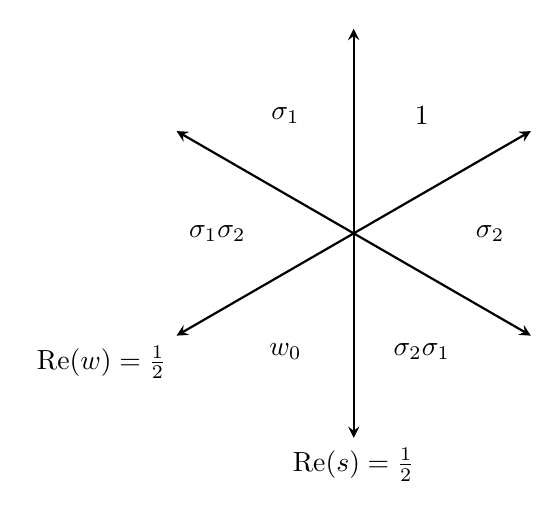
\begin{tikzpicture}[scale=3]
            \draw[thick,-stealth] (0:0) to (30:{sqrt(3)/2});
            \draw[thick,-stealth] (0:0) to (30:{-sqrt(3)/2}) node [below left] {$\Re(w) = \frac{1}{2}$};
            \draw[thick,-stealth] (0:0) to (90:{sqrt(3)/2});
            \draw[thick,-stealth] (0:0) to (90:{-sqrt(3)/2}) node [below] {$\Re(s) = \frac{1}{2}$};
            \draw[thick,-stealth] (0:0) to (150:{sqrt(3)/2});
            \draw[thick,-stealth] (0:0) to (150:{-sqrt(3)/2});

            \node at (60:{sqrt(3)/3}) {$1$};
            \node at (120:{sqrt(3)/3}) {$\s_{1}$};
            \node at (180:{sqrt(3)/3}) {$\s_{1}\s_{2}$};
            \node at (240:{sqrt(3)/3}) {$w_{0}$};
            \node at (300:{sqrt(3)/3}) {$\s_{2}\s_{1}$};
            \node at (0:{sqrt(3)/3}) {$\s_{2}$};
        \end{tikzpicture}
    \end{center}

    In the diagram, we we have shifted the $(s,w)$-plane so that the origin lies at $\left(\frac{1}{2},\frac{1}{2}\right)$ and we have tiled the $(s,w)$-axes so that they are no longer perpendicular. The effect of these adjustments is that $\s_{1}$ and $\s_{2}$ act by rigid motions sending the region enclosing $1$ (corresponding to the identity) to either of the adjacent triangles. The other regions are obtained by acting by the corresponding element of $W$. The initial region $\L$ that $Z(s,w)$ is defined on is displayed in the figure below:
    
    \begin{center}
        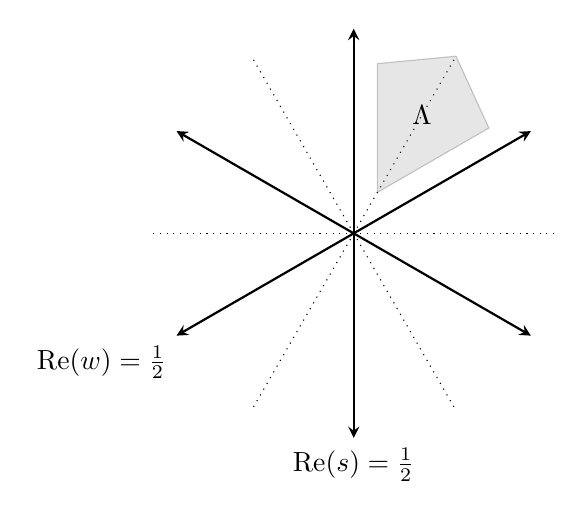
\begin{tikzpicture}[scale=3]
            \draw[dotted](0,0) to (60:{sqrt(3)/2});
            \draw[dotted](0,0) to (240:{sqrt(3)/2});
            \draw[dotted](0,0) to (180:{sqrt(3)/2});
            \draw[dotted](0,0) to (360:{sqrt(3)/2});
            \draw[dotted] (0:0) to (120:{sqrt(3)/2});
            \draw[dotted] (0:0) to (300:{sqrt(3)/2});

            \draw[thick,-stealth] (0:0) to (30:{sqrt(3)/2});
            \draw[thick,-stealth] (0:0) to (30:{-sqrt(3)/2}) node [below left] {$\Re(w) = \frac{1}{2}$};
            \draw[thick,-stealth] (0:0) to (90:{sqrt(3)/2});
            \draw[thick,-stealth] (0:0) to (90:{-sqrt(3)/2}) node [below] {$\Re(s) = \frac{1}{2}$};
            \draw[thick,-stealth] (0:0) to (150:{sqrt(3)/2});
            \draw[thick,-stealth] (0:0) to (150:{-sqrt(3)/2});


            \draw[fill=gray,opacity=0.2] (60:0.2) --+ (0,{((sqrt(5)/3)-0.2)}) -- (60:{sqrt(3)/2}) -- ($(60:0.2)+(30:{((sqrt(5)/3)-0.2)})$) -- cycle;

            \node at (60:{sqrt(3)/3}) {$\L$};
        \end{tikzpicture}
    \end{center}
    
     To meromorphically continue $Z(s,w)$ to all of the $(s,w)$-plane, we first need to analytically continue the double Dirichlet series $Z(s,w)$ and $Z_{1,\t}(s,w)$ to a slightly larger region than $\L$. This continuation will be achieved by the Phragm\'en-Lindel\"of convexity principal. Fix some small $\e > 0$. The functional equations for $L^{\ast}(s,\what{\chi}_{f_{0}})$ and $L^{\ast}(w,\what{\chi}_{g_{0}})$ provide the estimates
    \[
        L(-\e,\what{\chi}_{f_{0}}) \ll |f|^{\frac{1}{2}+\e} \quad \text{and} \quad L(-\e,\what{\chi}_{g_{0}}) \ll |g|^{\frac{1}{2}+\e},
    \]
    because $L(1+\e,\what{\chi}_{f_{0}}) \ll 1$ and $L(1+\e,\what{\chi}_{g_{0}}) \ll 1$. Since both of these $L$-functions at most have a simple pole at $s = 1$ and $w = 1$ respectively, the Phragm\'en-Lindel\"of convexity principal implies the weak estimates
    \[
        (s-1)L(s,\what{\chi}_{f_{0}}) \ll |f|^{\frac{1}{2}+\e} \quad \text{and} \quad (w-1)L(w,\what{\chi}_{g_{0}}) \ll |g|^{\frac{1}{2}+\e},
    \]
    for $\Re(s) > -\e$ and $\Re(w) > -\e$. But then from the interchange we see that $(s-1)(w-1)Z(s,w)$ and $(s-1)(w-1)Z_{1,\t}(s,w)$ are absolutely uniformly convergent on compacta on the region
    \[
        \L_{0} = \L \cup \left\{(s,w) \in \C^{2}:\Re(s) > 0, \Re(w) > \frac{3}{2}\right\} \cup \left\{(s,w) \in \C^{2}:\Re(s) > \frac{3}{2}, \Re(w) > 0\right\}.
    \]
    
    \begin{center}
        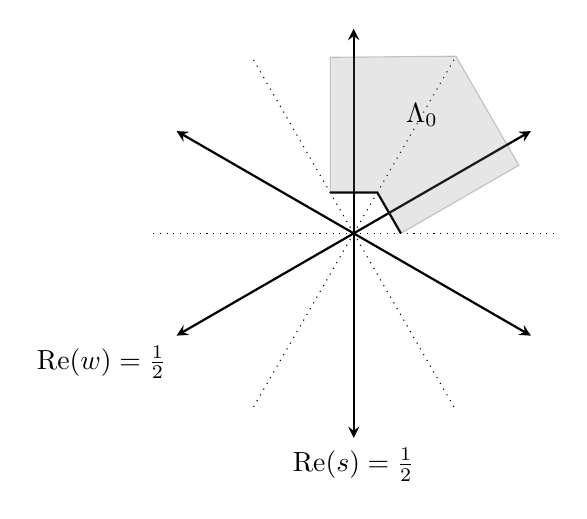
\begin{tikzpicture}[scale=3]
            \draw[dotted](0,0) to (60:{sqrt(3)/2});
            \draw[dotted](0,0) to (240:{sqrt(3)/2});
            \draw[dotted](0,0) to (180:{sqrt(3)/2});
            \draw[dotted](0,0) to (360:{sqrt(3)/2});
            \draw[dotted] (0:0) to (120:{sqrt(3)/2});
            \draw[dotted] (0:0) to (300:{sqrt(3)/2});

            \draw[thick,-stealth] (0:0) to (30:{sqrt(3)/2});
            \draw[thick,-stealth] (0:0) to (30:{-sqrt(3)/2}) node [below left] {$\Re(w) = \frac{1}{2}$};
            \draw[thick,-stealth] (0:0) to (90:{sqrt(3)/2});
            \draw[thick,-stealth] (0:0) to (90:{-sqrt(3)/2}) node [below] {$\Re(s) = \frac{1}{2}$};
            \draw[thick,-stealth] (0:0) to (150:{sqrt(3)/2});
            \draw[thick,-stealth] (0:0) to (150:{-sqrt(3)/2});

            \draw[thick] (0:0.2) -- (60:0.2) -- (120:0.2);

            \draw[fill=gray,opacity=0.2] (0:0.2) --+ (30:{cos(30)*((sqrt(3)/2)-0.2)}) -- (60:{sqrt(3)/2}) -- ($(120:0.2)+(0,{sqrt(5)/3-sin(120)*0.2})$) -- (120:0.2) -- (60:0.2) -- cycle;

            \node at (60:{sqrt(3)/3}) {$\L_{0}$};
        \end{tikzpicture}
    \end{center}
    
    In particular, $Z(s,w)$ and $Z_{1,\t}(s,w)$ are meromorphic on this region with at most polar lines at $s = 1$ and $w = 1$. The advantage of the region $\L_{0}$ over the intital region $\L$ is that $\L_{0}$ intersects the hyperplains $s = \frac{1}{2}$ and $w = \frac{1}{2}$ so that the union of the reflections $w\L_{0}$ for $w \in \W$ is connected. The idea now is to reflect $\L_{0}$ via the functional equations and then apply a theorem of Bochner. To state this theorem we need a small definition. We say that a domain $\W \subset \C^{n}$ is a \textbf{tube domain} if there is an open set $\w \subset \R^{n}$ such that
    \[
        \W = \{(s_{1},\ldots,s_{n}) \in \C^{n}:\Re((s_{1},\ldots,s_{n})) \in \w\}.
    \]
    Tube domains are generalizations of vertical strips in the complex plane. Now we can state the theorem of Bochner (see \cite{H} for a proof):

    \begin{theorem}[Bochner's continuation theorem]
        If $\W$ is a connected tube domain, then any holomorphic function on $\W$ can be extended to a holomorphic functon on the convex hull $\what{\W}$.
    \end{theorem}

    By clearing polar divisors, Bochner's continuation theorem implies that any meromorphic function on a connected tube domain posessing a finite amount of hyperplane polar divisors can be extended to a meromorphic function on the convex hull. This is exactly the situation for $Z(s,w)$. Indeed, it is clear that a union of tube domains is a tube domain and so, in particular, $\L_{0}$ is a tube domain. But on $\L_{0}$ there are a most polar lines at $s = 1$ and $w = 1$. Reflecting these hyperplanes via $W$ we obtain the finite set of possible polar divisors:
    \[
        \left\{s = 1, w = 1, s = 0, w = 0, s+w = \frac{1}{2}, s+w = \frac{3}{2}\right\}.
    \]
    Therefore we are reduced to extending $Z(s,w)$ meromorphically. By applying the functional equations corresponding to $\s_{1}$, $\s_{2}$, and $\s_{1}\s_{2}$, $Z(s,w)$ admits meromorphic continuation to the region
    \[
        \L_{12} = \L_{0} \cup \s_{1}\L_{0} \cup \s_{2}\L_{0} \cup \s_{1}\s_{2}\L_{0}.
    \]

    \begin{center}
        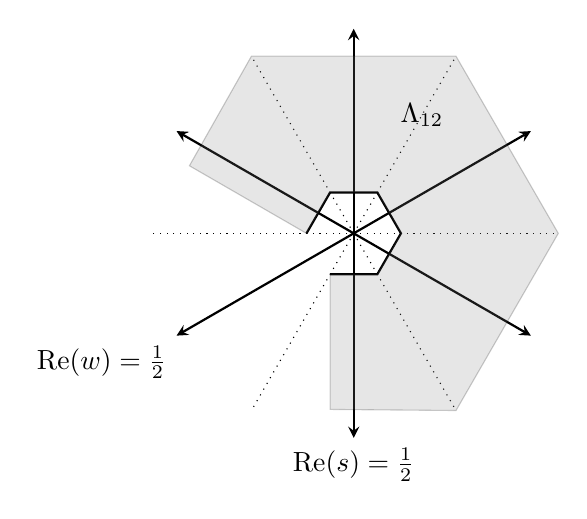
\begin{tikzpicture}[scale=3]
            \draw[dotted](0,0) to (60:{sqrt(3)/2});
            \draw[dotted](0,0) to (240:{sqrt(3)/2});
            \draw[dotted](0,0) to (180:{sqrt(3)/2});
            \draw[dotted](0,0) to (360:{sqrt(3)/2});
            \draw[dotted] (0:0) to (120:{sqrt(3)/2});
            \draw[dotted] (0:0) to (300:{sqrt(3)/2});

            \draw[thick,-stealth] (0:0) to (30:{sqrt(3)/2});
            \draw[thick,-stealth] (0:0) to (30:{-sqrt(3)/2}) node [below left] {$\Re(w) = \frac{1}{2}$};
            \draw[thick,-stealth] (0:0) to (90:{sqrt(3)/2});
            \draw[thick,-stealth] (0:0) to (90:{-sqrt(3)/2}) node [below] {$\Re(s) = \frac{1}{2}$};
            \draw[thick,-stealth] (0:0) to (150:{sqrt(3)/2});
            \draw[thick,-stealth] (0:0) to (150:{-sqrt(3)/2});

            \draw[thick] (240:0.2) -- (300:0.2) -- (0:0.2) -- (60:0.2) -- (120:0.2) -- (180:0.2);

            \draw[fill=gray,opacity=0.2] (240:0.2) --+ (0,{-((sqrt(5)/3)+sin(240)*0.2)}) -- (300:{sqrt(3)/2}) -- (0:{sqrt(3)/2}) -- (60:{sqrt(3)/2}) -- (120:{sqrt(3)/2}) -- ($(180:0.2)+(150:{((sqrt(5)/3)+cos(150)*0.2)})$) -- (180:0.2) -- (120:0.2) -- (60:0.2) -- (0:0.2)-- (300:0.2) -- cycle;

            \node at (60:{sqrt(3)/3}) {$\L_{12}$};
        \end{tikzpicture}
    \end{center}

    Because the functional equation for $Z(s,w)$ involves both $Z(s,w)$ and $Z_{1,\psi}(s,w)$, it was necessarily to analytically continue both of these double Dirichlet series to $\L_{0}$ before we applied the functional equation. Now $\L_{12}$ is a connected tube domain whose convex hull is $\C^{2}$. So by applying Bochner's continuation theorem (or rather our comment for meromorphic functions) we see that $Z(s,w)$ admits meromorphic continuation to the $(s,w)$-plane with at most a finite set of polar divisors. This method is better than repeatedly applying the functional equations corresponding to every $w \in W$. Indeed, if we did we would obtain meromorphic continuation to the region
    \[
        \L_{W} = \bigcup_{w \in W} w\L_{0}.
    \]

    \begin{center}
        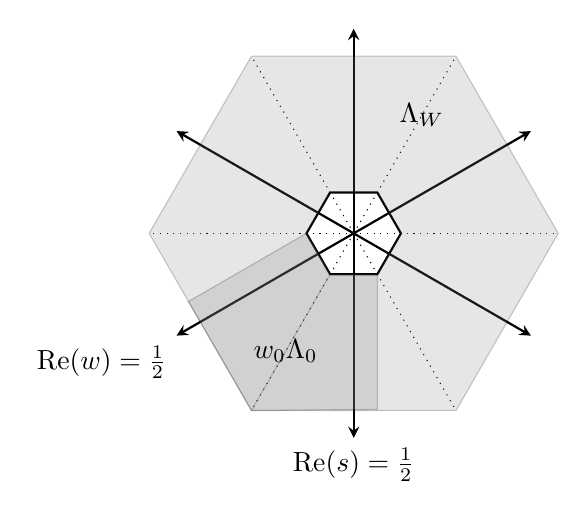
\begin{tikzpicture}[scale=3]
            \draw[dotted](0,0) to (60:{sqrt(3)/2});
            \draw[dotted](0,0) to (240:{sqrt(3)/2});
            \draw[dotted](0,0) to (180:{sqrt(3)/2});
            \draw[dotted](0,0) to (360:{sqrt(3)/2});
            \draw[dotted] (0:0) to (120:{sqrt(3)/2});
            \draw[dotted] (0:0) to (300:{sqrt(3)/2});

            \draw[thick,-stealth] (0:0) to (30:{sqrt(3)/2});
            \draw[thick,-stealth] (0:0) to (30:{-sqrt(3)/2}) node [below left] {$\Re(w) = \frac{1}{2}$};
            \draw[thick,-stealth] (0:0) to (90:{sqrt(3)/2});
            \draw[thick,-stealth] (0:0) to (90:{-sqrt(3)/2}) node [below] {$\Re(s) = \frac{1}{2}$};
            \draw[thick,-stealth] (0:0) to (150:{sqrt(3)/2});
            \draw[thick,-stealth] (0:0) to (150:{-sqrt(3)/2});

            \draw[thick] (240:0.2) -- (300:0.2) -- (0:0.2) -- (60:0.2) -- (120:0.2) -- (180:0.2) -- cycle;
        
            \draw[fill=gray,opacity=0.2] (240:{sqrt(3)/2}) -- (300:{sqrt(3)/2}) -- (0:{sqrt(3)/2}) -- (60:{sqrt(3)/2}) -- (120:{sqrt(3)/2}) -- (180:{sqrt(3)/2}) -- (240:{sqrt(3)/2}) -- (240:0.2) -- (180:0.2) -- (120:0.2) -- (60:0.2) -- (0:0.2) -- (300:0.2) -- (240:0.2) -- cycle;

            \draw[fill=gray,opacity=0.2] (180:0.2) --+ (210:{-cos(210)*((sqrt(3)/2)-0.2)}) -- (240:{sqrt(3)/2}) -- ($(300:0.2)+(0,{-((sqrt(5)/3)+sin(300)*0.2)})$) -- (300:0.2) -- (240:0.2) -- cycle; 

            \node at (60:{sqrt(3)/3}) {$\L_{W}$};
            \node at (240:{sqrt(3)/3}) {$w_{0}\L_{0}$};
        \end{tikzpicture}
    \end{center}
    
    There are two issues here. The first is that $Z(s,w)$ has two meromorphic continuations to the region $w_{0}\L_{0}$ given by the functional equations corresponding to $w_{0} = \s_{1}\s_{2}\s_{1}$ and $w_{0} = \s_{2}\s_{1}\s_{2}$ and we would need to show that these agree. The second is that we have not obtained meromorphic continuation to $\C^{2}-\L_{W}$ which is a compact hexagon about the origin. By using Bochner's theorem after meromorphically continuning to $\L_{12}$, we have avoided these issues and as a consquence shown that the meromorphic continuations given by $w_{0} = \s_{1}\s_{2}\s_{1}$ and $w_{0} = \s_{2}\s_{1}\s_{2}$ agree.
\section{Poles and Residues}
    We will inespect the polar divisors of $Z(s,w)$ more carefully. It turns out that the set of polar divisors is smaller than
    \[
        \left\{s = 1, w = 1, s = 0, w = 0, s+w = \frac{1}{2}, s+w = \frac{3}{2}\right\}.
    \]
    Indeed, there are no poles on the hyperplanes $s = 0$, $w = 0$, and $s+w = \frac{3}{2}$. To see this, first note that by our earlier application of the Phragm\'en-Lindel\"of convexity principal we actually obtained continuation to an open set containing $\L_{0}$ (because our estimates held for $\Re(s) > -\e$ and $\Re(w) > -\e$). We did not need this larger region for the meromorphic continuation but we do need it to study the poles. Now consider the possible polar divisor $s = 0$. We know $(s-1)(w-1)Z(s,w)$ and $(s-1)(w-1)Z_{1,\t}(s,w)$ are holomorphic on an open set containing $\L_{0}$ which contains half of the hyperplane defined by $s = 0$ outside of the hexagon $\C^{2}-\L_{W}$. As $(s-1)(w-1)$ is holomorphic on this region it follows that $Z(s,w)$ and $Z_{1,\t}(s,w)$ do not have a polar divisor at $s = 0$ on an open set containing $\L_{0}$. Now note that an open set containing $\s_{1}\s_{2}\L_{0}$ contains the other half of the hyperplane defined by $s = 0$ outside of the hexagon $\C^{2}-\L_{W}$. Upon applying the functional equation corresponding to $\s_{1}\s_{2}$, \cref{thm:double_Dirichlet_series_functional_equation} implies that the gamma factors in the corresponding functional equation have a simple pole when $s+w = \frac{3}{2}$ (the gamma factors in the functional equation for $\s_{1}$ have a simple pole at $s = 1$ and $s-1 \to s+w-\frac{3}{2}$ under $\s_{2}$). Therefore $Z(s,w)$ and $Z_{1,\t}(s,w)$ do not have polar divisors at $s = 0$ on an open set containing $\s_{1}\s_{2}\L_{0}$ away from $s+w = \frac{3}{2}$. In particular, $Z(s,w)$ does not have a polar divisor at $s = 0$ on $\L_{W}$ and away from the other polar divisors. By Bochner's continuation theorem (after clearing all of the other possible polar divisors), we see that $Z(s,w)$ does not have a polar divisors at $s = 0$ on all of $\C^{2}$ and away from the other polar divisors. An identical argument holds for the case $w = 0$ with the regions $\L_{0}$ and $\s_{2}\s_{1}\L_{0}$. For the polar divisor $s+w = \frac{1}{2}$, we argue in the same way with the regions $\s_{2}\s_{1}\L_{0}$, $\s_{1}\s_{2}\L_{0}$, and $w_{0}\L_{0}$. The only difference is that for these regions the gamma factors in the corresponding functional equations are different. For the first two regions $\s_{2}\s_{1}\L_{0}$ and $\s_{1}\s_{2}\L_{0}$ the gamma factors have a simple pole when $s+w = \frac{3}{2}$. For the third region $w_{0}\L_{0}$ the gamma factors have simple poles at $s = 1$ and $w = 1$ which is seen by using both representations $w_{0} = \s_{1}\s_{2}\s_{1}$ and $w_{0} = \s_{2}\s_{1}\s_{2}$. So in conclusion, there are no poles on the hyperplanes $s = 0$, $w = 0$, and $s+w = \frac{1}{2}$ and away from the other polar divisors. As for the hyperplanes $s = 1$, $w = 1$, and $s+w = \frac{3}{2}$, there are clearly genuine poles for $s = 1$ and $w = 1$ coming from $L(s,\chi_{f_{0}})$ and $L(w,\chi_{g_{0}})$ when $f$ and $g$ are perfect squares (so that $f_{0} = g_{0} = 1$). For $s+w = \frac{3}{2}$, we have a pole coming from the gamma factors corresponding to the functional equations for $\s_{2}\s_{1}$ and $\s_{1}\s_{2}$. We collect all of our work as a theorem:

    \begin{theorem}
        $Z(s,w)$ admits meromorphic continuation to $\C^{2}$ with polar divisors $s = 1$, $w = 1$, and $s+w = \frac{3}{2}$.
    \end{theorem}

    We can now look at the residue of $Z(s,w)$ at these poles. Since all of the poles are obtained from each other by applying the functional equations of $Z(s,w)$, we begin by looking at the pole at $w = 1$. We assume $s \neq \frac{1}{2}$ to ensure that we are not looking at a point that is an intersection of two polar lines. This case will be inspected in a moment. To compute the residue we use the representation
    \[
        Z(s,w) = \sum_{\text{$g$ monic}}\frac{L(w,\chi_{g_{0}})Q_{g_{0}g_{1}^{2}}(w)}{|g|^{s}},
    \]
    coming from the interchange. For a fixed $g$, the numerator $L(w,\chi_{g_{0}})Q_{g_{0}g_{1}^{2}}(w)$ in the summand corresponding to $g$ has a pole at $w = 1$ if and only if $g_{0}$ is square-free, that is $g_{0} = 1$, or equivalently $g = g_{1}^{2}$ itself is a perfect square. In this case, $L(w,\chi_{g_{0}}) = \z(w)$ so that
    \[
        \Res_{w = 1}L(w,\chi_{g_{0}})Q_{g_{0}g_{1}^{2}}(w) = \frac{1}{\log(q)}Q_{g_{1}^{2}}(1).
    \]
    But from \cref{lem:prime_correction_even,thm:correction_polynomial_Euler_product} we see that $Q_{g_{1}^{2}}(1) = 1$, and so
    \[
        \Res_{w = 1}Z(s,w) = \frac{1}{\log(q)}\sum_{\text{$g$ monic perfect square}}\frac{Q_{g_{1}^{2}}(1)}{|g|^{s}} = \frac{1}{\log(q)}\sum_{\text{$g$ monic}}\frac{1}{|g|^{2s}} = \frac{1}{\log(q)}\z(2s).
    \]
    The residue at $s = 1$, provided $w \neq \frac{1}{2}$, is immediate from what we have done so far. Indeed, by applying the interchange, the exact same argument holds with the roles of $s$ and $w$ interchanged so that
    \[
        \Res_{s = 1}Z(s,w) = \frac{1}{\log(q)}\z(2w).
    \]
    The other reisdues of the simple poles can be computed by apply the functional equations for $Z(s,w)$ and using the resiudes at $s = 1$ and $w = 1$.

    Now we will investiage the points where the polar lines $w = 1$ and $s+w = \frac{1}{2}$ intersect. What we mean by this is we want to understand the polar structure of $Z\left(\frac{1}{2},w\right)$ at $w = 1$. To acomplish this, the Mittag-Leffler theorem applied to $Z(s,w)$ (in $w$) implies that
    \[
        Z(s,w) = \frac{R_{1}(s)}{w-1}+\frac{R_{2}(s)}{s+w-\frac{3}{2}}+Y(s,w),
    \]
    in some neighborhood of $\left(\frac{1}{2},1\right)$ where $Y(s,w)$ is holomorphic on this neighborhood and we have set
    \[
        R_{1}(s) = \Res_{w = 1}Z(s,w) \quad \text{and} \quad R_{2}(s) = \Res_{w = \frac{3}{2}-s}Z(s,w).
    \]
    From our residue computations, $R_{1}(s) = \frac{1}{\log(q)}\z(2s)$ which implies that it has a simple pole at $s = \frac{1}{2}$. The reisdue is given by $A = \frac{1}{2\log(q)}$. On the other hand, $Z\left(\frac{1}{2},w\right)$ is holomorphic for $\Re(w) > 1$. These two facts together imply that $R_{2}(s)$ must have a simple pole at $s = \frac{1}{2}$ which cancels the simple pole coming from $R_{1}(s)$. So by Mittag-Leffler again, we may write
    \[
        R_{1}(s) = \frac{A}{s-\frac{1}{2}}+R_{3}(s) \quad \text{and} \quad R_{2}(s) = -\frac{A}{s-\frac{1}{2}}+R_{4}(s).
    \]
    It follows that
    \begin{align*}
        Z(s,w) &= \frac{R_{1}(s)}{w-1}+\frac{R_{2}(s)}{s+w-\frac{3}{2}}+Y(s,w) \\ 
        &= \frac{A}{(w-1)\left(s-\frac{1}{2}\right)}+\frac{R_{3}(s)}{w-1}-\frac{A}{\left(s+w-\frac{3}{2}\right)\left(s-\frac{1}{2}\right)}+\frac{R_{4}(s)}{s+w-\frac{3}{2}}+Y(s,w) \\
        &= \frac{A}{(w-1)\left(s+w-\frac{3}{2}\right)}+\frac{R_{3}(s)}{w-1}+\frac{R_{4}(s)}{s+w-\frac{3}{2}}+Y(s,w).
    \end{align*}
    We can now set $s = \frac{1}{2}$ and let $B = R_{3}\left(\frac{1}{2}\right)+R_{4}\left(\frac{1}{2}\right)$ so that
    \[
        Z\left(\frac{1}{2},w\right) = \frac{A}{(w-1)^{2}}+\frac{B}{w-1}+O(1).
    \]
    It follows that $Z\left(\frac{1}{2},w\right)$ has a double pole at $w = 1$. This can be thought of as follows: the polar lines $w = 1$ and $s+w = \frac{3}{2}$ correspond to simple poles of $Z(s,w)$ except in the case when they intersect and the order of the poles combine to give a $Z\left(\frac{1}{2},w\right)$ a double pole at $w = 1$. Applying the interchange, the exact same argument holds to show that $Z(s,\frac{1}{2})$ has a double pole at $s = 1$.
\section*{\texorpdfstring{$Z(s,w)$}{Z(s,w)} as a Rational Function}
    Recall that $L(s,\chi_{f})$ is a polynomial in $q^{-s}$ of degree at most $\deg(f)-1$. A similar situation happens for the double Dirichlet series $Z(s,w)$, it will be a rational function in the variables $x = q^{-s}$ and $y = q^{-w}$. Since this property is a special case of Dirichlet series over function fields, we present the argument but supress the more detailed computations. Before we begin, we recall some properties of Hadamard products of power series. The details can be found in \cite{S}. For any two power series
    \[
        R_{1}(x,y) = \sum_{n,m \ge 0}r_{1}(n,m)x^{n}y^{m} \quad \text{and} \quad R_{2}(x,y) = \sum_{n,m \ge 0}r_{2}(n,m)x^{n}y^{m},
    \]
    or more generally generating series, their \textbf{Hadamard product} $(R_{1} \ast R_{2})(x,y)$ is defined by
    \[
        (R_{1} \ast R_{2})(x,y) = \sum_{n,m \ge 0}r_{1}(n,m)r_{2}(n,m)x^{n}y^{m}.
    \]
    If we assume $R_{1}(x,y)$ and $R_{2}(x,y)$ are regular around the origin $x = y = 0$, then the Hadamard product can be expressed as two contour integrals around the origin:
    \[
        (R_{1} \ast R_{2})(x,y) = \frac{1}{(2\pi i)^{2}}\int_{|z| = \rho}\int_{|w| = \rho}R_{1}(z,w)R_{2}\left(\frac{x}{z},\frac{y}{w}\right)\,\frac{dz}{z}\,\frac{dw}{w},
    \]
    for sufficiently small $\rho > 0$. By the residue theorem,
    \[
        (R_{1} \ast R_{2})(x,y) = \sum_{s = s(x,y)}\Res_{s}\left(R_{1}(z,w)R_{2}\left(\frac{x}{z},\frac{y}{w}\right)\frac{1}{zw}\right),
    \]
    where the sum is over all poles $s = s(x,y)$ of the integrand such that $\lim_{x,y \to 0}s(x,y) = 0$. This formula can be used to compute the Hadamard product of rational functions and in the following arguemnt where computing a Hadamard product is necessary, this method can be used.

    Now we show that $Z(s,w)$ is a rational function in $x = q^{-s}$ and $y = q^{-w}$. Throughout, we work in the region of absolute uniform convergence on compacta for $Z(s,w)$. Consider the representation
    \[
        Z(s,w) = \sum_{\text{$f$ monic}}\frac{L(s,\what{\chi}_{f_{0}})}{|f|^{w}} = \sum_{\text{$f,g$ monic}}\frac{\chi_{f_{0}}(\what{g})a(f,g)}{|f|^{w}|g|^{s}}.
    \]
    Since $L(s,\chi_{f})$ is a polynomial in $q^{-s}$ of degree at most $\deg(f)-1$ and correction polynomials $Q_{f_{0}f_{1}^{2}}(s)$ are Dirichlet polynomials, one of the two following cases occur:
    \begin{itemize}
        \item If $f$ is a perfect square, then $L(s,\chi_{f_{0}}) = \z(s)$ and
        \[
            L(s,\what{\chi}_{f_{0}}) = \z(s)Q_{f_{1}^{2}}(s),
        \]
        where $Q_{f_{1}^{2}}(s)$ is a polynomial in $q^{-s}$ of degree $\deg(f)$.
        \item If $f$ is not a perfect square, then
        \[
            L(s,\what{\chi}_{f_{0}}) = L(s,\chi_{f_{0}})Q_{f_{0}f_{1}^{2}}(s),
        \]
        is a polynomial in $q^{-s}$ of degree at most $\deg(f)-1$.
    \end{itemize}
    So if $f$ is not a perfect square, then
    \[
        L(s,\what{\chi}_{f_{0}}) = \sum_{\deg(g) \le \deg(f)-1}\frac{\chi_{f_{0}}(\what{g})a(f,g)}{|g|^{s}},
    \]
    which is to say that
    \[
        \sum_{\deg(g) = m}\chi_{f_{0}}(\what{g})a(f,g) = 0,
    \]
    for every $m \ge \deg(f)$ provided $f$ is not a perfect square. To exploit this fact, we will decompose $Z(s,w)$ according to whether $\deg(f) \ge \deg(g)$ or $\deg(f) \le \deg(g)$. So we write
    \[
        Z(s,w) = Z_{0}(s,w)+Z_{0}(w,s)-Z_{1}(s,w),
    \]
    where
    \[
        Z_{0}(s,w) = \sum_{0 \le n \le m}\frac{1}{q^{nw}q^{ms}}\sum_{\substack{\text{$f,g$ monic} \\ \deg(f) = n \\ \deg(g) = m}}\chi_{f_{0}}(\what{g})a(f,g) \quad \text{and} \quad Z_{1}(s,w) = \sum_{n \ge 0}\frac{1}{q^{nw}q^{ns}}\sum_{\substack{\text{$f,g$ monic} \\ \deg(f) = n \\ \deg(g) = n}}\chi_{f_{0}}(\what{g})a(f,g).
    \]
    We will now show that $Z_{0}(s,w)$ and $Z_{1}(s,w)$ are rational functions in $q^{-s}$ and $q^{-w}$ via a convolution procedure. For $Z_{0}(s,w)$, our remarks about $L(s,\what{\chi}_{f_{0}})$ imply the term in the inner sum of $Z_{0}(s,w)$ vanishes unless $f$ is a perfect square and in this case $\chi_{f_{0}}(\what{g}) = 1$. Therefore
    \[
        Z_{0}(s,w) = \sum_{0 \le n \le m}\frac{1}{q^{nw}q^{ms}}\sum_{\substack{\text{$f,g$ monic} \\ \text{$f$ a perfect square} \\ \deg(f) = n \\ \deg(g) = m}}a(f,g).
    \]
    Now consider
    \[
        Y(s,w) = \sum_{\substack{\text{$f,g$ monic} \\ \text{$f$ monic perfect square}}}\frac{a(f,g)}{|f|^{s}|g|^{w}} \quad \text{and} \quad K_{0}(s,w) = \sum_{0 \le n \le m}\frac{1}{q^{nw}q^{ms}}.
    \]
    We can express both of these as rational functions in $q^{-s}$ and $q^{-w}$. Indeed, for $Y(s,w)$, \cref{prop:multiplicativity_of_weighting_coefficients}  we that $Y(s,w)$ posesses a Euler product. Using \cref{cor:evaulation_of_weighting_coefficients_at_primes}, we compute
    \[
        Y(s,w) = \frac{1-q^{1-s-2w}}{(1-q^{1-2w})(1-q^{1-s})(1-q^{2-2s-2w})},
    \]
    which can also be seen by comparing coefficients of the power series expansion of the right-hand side. $K_{0}(s,w)$ is even easier because it is a geometric series:
    \[
        K_{0}(s,w) = \sum_{0 \le n \le m}\frac{1}{q^{nw}q^{ms}} = \frac{1}{(1-q^{-s})(1-q^{-s-w})}.
    \]
    Then $Z_{0}(s,w)$ is expressed as a Hadamard product of power series in $q^{-s}$ and $q^{-w}$:
    \[
        Z_{0}(s,w) = Y(s,w) \ast K_{0}(s,w).
    \]
    Then using the countour integral representation of the Hadamard product, we compute
    \[
        Z_{0}(s,w) = \frac{1}{(1-q^{1-s})(1-q^{3-2s-2w})}.
    \]
    For $Z_{1}(s,w)$, our remarks about $L(s,\what{\chi}_{f_{0}})$ similarly imply
    \[
        Z_{1}(s,w) = \sum_{n \ge 0}\frac{1}{q^{ns}q^{nw}}\sum_{\substack{\text{$f,g$ monic} \\ \text{$f$ a perfect square} \\ \deg(f) = n \\ \deg(g) = n}}a(f,g).
    \]
    But then we may repeat the same argument as for $Z_{0}(s,w)$ with
    \[
        Y(s,w) = \sum_{\substack{\text{$f,g$ monic} \\ \text{$f$ monic perfect square}}}\frac{a(f,g)}{|f|^{s}|g|^{w}} \quad \text{and} \quad K_{1}(s,w) = \sum_{n \ge 0}\frac{1}{q^{ns}q^{nw}},
    \]
    and arrive at
    \[
        Z_{1}(s,w) = \frac{1}{(1-q^{3-2s-2w})}.
    \]
    Combining these representations for $Z_{0}(s,w)$ and $Z_{1}(s,w)$ with our decomposition of $Z(s,w)$ yields
    \[
        Z(s,w) = \frac{1-q^{2-s-w}}{(1-q^{1-s})(1-q^{1-w})(1-q^{3-2s-2w})}.
    \]
    Setting $x = q^{-s}$ and $y = q^{-w}$ gives
    \[
        Z(x,y) = \frac{1-q^{2}xy}{(1-qx)(1-qy)(1-q^{3}x^{2}y^{2})},
    \]
    which is a rational function in $x$ and $y$.

    \begin{remark}
        Some authors, especially those using the Chinta-Gunnells construction of building multiple Dirichlet series, prefer the $W$-invariant point to be at the origin. For this, we make the change of variables $\left(s+\frac{1}{2},w+\frac{1}{2}\right) \to (s,w)$ which gives
        \[
            Z(s,w) = \frac{1-q^{1-s-w}}{(1-q^{\frac{1}{2}-s})(1-q^{\frac{1}{2}-w})(2-q^{3-2s-2w})},
        \]
         and upon setting $x = q^{-s}$ and $y = q^{-w}$, we have
        \[
            Z(x,y) = \frac{1-qxy}{(1-q^{\frac{1}{2}}x)(1-q^{\frac{1}{2}}y)(1-q^{2}x^{2}y^{2})}.
        \]
    \end{remark}

\begin{thebibliography}{99}
    \bibitem{R}
    Rosen, M. (2002). Number theory in function fields (Vol. 210). Springer Science \& Business Media.

    \bibitem{H}
    Hormander, L. (1973). An introduction to complex analysis in several variables. Elsevier.

    \bibitem{CG}
    Chinta, G., \& Gunnells, P. E. (2007). Weyl group multiple Dirichlet series constructed from quadratic characters. Inventiones mathematicae, 167, 327-353.

    \bibitem{S}
    Stanley, R. (2023). Enumerative Combinatorics: Volume 2. Cambridge University Press.
\end{thebibliography}

\end{document}